%% Manuscript for Intelligent Service Robotics (Springer). Springer Nature LaTeX template (sn-jnl.cls,
%% obtained from Springer Nature's LaTeX author support page; not redistributed here, see README.md).
%% Every number in the text is a macro generated from the stored results by
%% tools/research/phase7/make_tables.py (tables/numbers.tex); none is typed by hand.
\documentclass[pdflatex,sn-mathphys-num]{sn-jnl}

\usepackage{graphicx}
\usepackage{amsmath,amssymb,amsfonts}
\usepackage{booktabs}
\usepackage{xcolor}
\usepackage{url}

% Generated by tools/research/phase7/make_tables.py from research/phase7/results. Do not edit.
\newcommand{\devParts}{151}
\newcommand{\devAllParts}{316}
\newcommand{\devNFMzero}{6.07}
\newcommand{\devNFMone}{1.25}
\newcommand{\devNegMone}{9}
\newcommand{\devWorstMone}{25}
\newcommand{\devNFMfour}{1.23}
\newcommand{\devNegMfour}{8}
\newcommand{\devWorstMfour}{11}
\newcommand{\devNFMnine}{1.29}
\newcommand{\devNegMnine}{11}
\newcommand{\devWorstMnine}{37}
\newcommand{\devNFJoint}{1.29}
\newcommand{\devNegJoint}{10}
\newcommand{\devWorstJoint}{10}
\newcommand{\devHybridNF}{1.32}
\newcommand{\devHybridWorst}{2}
\newcommand{\devRobustMzero}{80.1}
\newcommand{\devLoadMzero}{58.9}
\newcommand{\devRobustVtwoMzero}{84.1}
\newcommand{\devLoadVtwoMzero}{64.9}
\newcommand{\devRobustMone}{84.8}
\newcommand{\devLoadMone}{45.0}
\newcommand{\devRobustVtwoMone}{90.7}
\newcommand{\devLoadVtwoMone}{48.3}
\newcommand{\devRobustMfour}{85.4}
\newcommand{\devLoadMfour}{55.0}
\newcommand{\devRobustVtwoMfour}{92.7}
\newcommand{\devLoadVtwoMfour}{60.3}
\newcommand{\devRobustMnine}{88.7}
\newcommand{\devLoadMnine}{39.1}
\newcommand{\devRobustVtwoMnine}{96.0}
\newcommand{\devLoadVtwoMnine}{46.4}
\newcommand{\devRobustJoint}{89.4}
\newcommand{\devLoadJoint}{56.3}
\newcommand{\devRobustVtwoJoint}{96.7}
\newcommand{\devLoadVtwoJoint}{62.3}
\newcommand{\devJointMzeroRobust}{+9.3}
\newcommand{\devJointMzeroRobustCI}{[2.6, 15.9]}
\newcommand{\devJointMzeroLoad}{-2.6}
\newcommand{\devJointMzeroLoadCI}{[-9.3, 4.0]}
\newcommand{\devJointMoneRobust}{+4.6}
\newcommand{\devJointMoneRobustCI}{[0.0, 9.3]}
\newcommand{\devJointMoneLoad}{+11.3}
\newcommand{\devJointMoneLoadCI}{[5.3, 17.2]}
\newcommand{\devMfourMoneLoad}{+9.9}
\newcommand{\devMfourMoneLoadCI}{[4.6, 15.9]}
\newcommand{\devMnineMoneRobust}{+4.0}
\newcommand{\devMnineMoneRobustCI}{[-0.7, 8.6]}
\newcommand{\devVtwoHeld}{3423}
\newcommand{\devVtwoNotVthree}{128}
\newcommand{\devTurnOverFifteen}{3.7}
\newcommand{\devFlipLow}{18.4}
\newcommand{\devFlipMid}{7.4}
\newcommand{\devFlipHigh}{6.1}
\newcommand{\artAgreeMin}{95}
\newcommand{\artAgreeMax}{97}
\newcommand{\artKappaMin}{0.74}
\newcommand{\artKappaMax}{0.82}
\newcommand{\artKappaTwoKg}{0.60}
\newcommand{\artHeldTwoKgVthree}{57}
\newcommand{\artHeldTwoKgArt}{40}
\newcommand{\artGrasps}{430}
\newcommand{\artJointMoneLoad}{-3.3}
\newcommand{\artJointMoneLoadCI}{[-10.6, 4.0]}
\newcommand{\artJointMzeroLoad}{-17.2}
\newcommand{\artJointMzeroLoadCI}{[-24.5, -10.6]}
\newcommand{\artJointMzeroRobust}{+8.0}
\newcommand{\artJointMzeroRobustCI}{[2.0, 13.9]}
\newcommand{\artTrackMax}{0.119}
\newcommand{\repAUCLzero}{0.9958}
\newcommand{\repNFLzero}{1.316}
\newcommand{\repNFLtwo}{1.494}
\newcommand{\repNFLten}{1.425}
\newcommand{\repLtwoLzero}{1.135}
\newcommand{\repLtwoLzeroCI}{[1.035, 1.248]}
\newcommand{\repLeightLtwo}{1.014}
\newcommand{\repLeightLtwoCI}{[0.969, 1.059]}
\newcommand{\repLeightPerm}{0.999}
\newcommand{\repLeightPermCI}{[0.955, 1.042]}
\newcommand{\repLtenLtwo}{0.954}
\newcommand{\repLtenLtwoCI}{[0.907, 0.998]}
\newcommand{\repLtenPerm}{0.945}
\newcommand{\repLtenPermCI}{[0.898, 0.995]}
\newcommand{\repLsevenLtwo}{0.989}
\newcommand{\repLsevenLtwoCI}{[0.944, 1.031]}
\newcommand{\repLelevenLtwo}{1.010}
\newcommand{\repLelevenLtwoCI}{[0.961, 1.060]}
\newcommand{\repLGLtwo}{0.932}
\newcommand{\repLGLtwoCI}{[0.872, 0.991]}
\newcommand{\repLDLtwo}{0.936}
\newcommand{\repLDLtwoCI}{[0.875, 1.001]}
\newcommand{\repRankLtwo}{1.007}
\newcommand{\repRankLtwoCI}{[0.940, 1.076]}
\newcommand{\repVisibleShare}{88}
\newcommand{\fewFirstShare}{87}
\newcommand{\fewCeiling}{1.30}
\newcommand{\fewCeilingMs}{5.2}
\newcommand{\fewFixedS}{0.57}
\newcommand{\crossForty}{0.94}
\newcommand{\crossFortyCI}{[0.74, 1.19]}
\newcommand{\crossFortyViable}{79}
\newcommand{\crossHundredtwenty}{1.07}
\newcommand{\crossHundredtwentyCI}{[0.99, 1.16]}
\newcommand{\crossHundredtwentyViable}{254}
\newcommand{\powerPtwo}{0.994}


\begin{document}

\title[Robustness-aware candidate ordering for a complete grasp planner]{Learning where to look first without losing robustness: a pre-registered evaluation of candidate ordering for a complete parallel-jaw grasp planner}

\author*{\fnm{Eduardo} \sur{P\'erez Gonz\'alez}}\email{[to be provided by the author]}

\affil*{\orgname{Independent Researcher}, \orgaddress{\city{Zaragoza}, \country{Spain}}}

\abstract{A complete grasp planner examines a catalogue of candidate grasps one by one---inverse kinematics, collisions, static wrench quality---and stops at the first feasible one. A classifier that predicts feasibility can reorder the catalogue so that far fewer candidates are examined, but the order it learns also decides which grasp is executed. We show, on \devParts{} household objects in simulation, that a learned feasibility order makes the planner reach a feasible grasp after \devNFMone{} instead of \devNFMzero{} candidates (geometric mean), and that it changes dynamic robustness and load tolerance. We propose FORTIS-R Joint, an order that multiplies the feasibility prior by a learned probability of dynamic robustness and by a centring term, and a round-robin fallback with a deterministic bound of twice the original planner's cost. Before testing, we corrected the physics (masses, centre of mass, in-hand rotation, torsional friction), ran an articulated-arm replication, measured frozen vision foundation-model features (DINOv2, DINOv3, OpenCLIP) against permuted and untrained controls, and froze the method, the hypotheses and the analysis. On \confObjects{} independently selected EGAD objects, FORTIS-R Joint examined \confPoneRatio{} times as many candidates as the original planner (\confPoneVerdict), its robustness relative to the original planner was \confPtwoDiff{} percentage points (non-inferiority \confPtwoVerdict), and its number of examined candidates relative to the best learned baseline was \confPthreeRatio{} (non-inferiority \confPthreeVerdict). Load-tolerance conclusions depended on the simulator level and on uncalibrated friction, and foundation-model features gave no development gain under the pre-declared rule. All results are simulation results, not robot experiments.}

\keywords{Grasp planning, Parallel-jaw grasping, Learning to order, Dynamic robustness, Pre-registration, Vision foundation models}

\maketitle

\section{Introduction}\label{sec:intro}

Service robots that pick previously unseen household objects must plan a grasp quickly and the grasp must hold. Sampling-based planners address the first need by generating a catalogue of candidate grasps and examining candidates until one passes every check \cite{bohg2014survey,newbury2023review}. Examining a candidate is the expensive part: inverse kinematics for the arm, collision checking of the approach and the grasp, and a static wrench-space quality test \cite{ferrari1992planning}. If the planner examines candidates in a poor order, it spends most of its time on candidates that fail.

Learning which candidates are likely to pass, and examining those first, is an established idea \cite{lou2020reachability,akinola2021dynamic,qin2025planned}. Two aspects of it are less studied. First, the order does not only decide how long planning takes; it also decides \emph{which} feasible grasp is returned, and therefore whether the grasp survives perturbations, heavier loads or in-hand rotation. Prior work has shown that grasps that score best on an analytic metric are not always the most robust \cite{weisz2012pose}; here the tension is between reaching feasibility quickly and dynamic robustness. Second, conclusions about learned orders are usually drawn on the data used to design them.

This article reports a controlled and pre-registered study of that tension for a complete parallel-jaw planner (AxisForge). Its contributions are:
\begin{enumerate}
\item an exact replay of the planner's own order arithmetic over exhaustively labelled catalogues, so that any order can be evaluated without re-planning (Sect.~\ref{sec:planner});
\item corrected dynamic validation in MuJoCo \cite{todorov2012mujoco}---intended masses, the planner's centre of mass, an in-hand rotation criterion, a torsional-friction grid and an articulated-arm replication---and the evidence that load-tolerance conclusions depend on those modelling choices (Sect.~\ref{sec:physics});
\item FORTIS-R Joint, a product of feasibility, learned robustness and a centring term, with a round-robin fallback whose cost is never more than twice that of the original order (Sect.~\ref{sec:methods});
\item a development study of frozen vision foundation-model features \cite{caron2021dino,oquab2024dinov2,simeoni2025dinov3,radford2021clip} with permuted, untrained and linear controls, local patch features at the contacts, and a ranking loss (Sect.~\ref{sec:dev});
\item an independent confirmation on EGAD \cite{morrison2020egad} with the method, the hypotheses, the sample size and the analysis frozen and signed by hashes before any confirmatory object was planned (Sect.~\ref{sec:conf}).
\end{enumerate}
We do not claim a new grasping algorithm: the components are known; the contribution is the controlled measurement and its confirmation. All experiments are in simulation.

\section{Related work}\label{sec:related}

\paragraph{Grasp synthesis.} Surveys distinguish analytic and data-driven synthesis and, among deep methods, sampling-based approaches, direct regression, reinforcement learning and exemplar methods \cite{bohg2014survey,newbury2023review}. Learned detectors such as Dex-Net 2.0 \cite{mahler2017dexnet2}, GPD \cite{tenpas2017gpd}, Contact-GraspNet \cite{sundermeyer2021contactgraspnet} and GraspNet-1Billion \cite{fang2020graspnet} score or generate grasps from sensor data. Eppner et al. showed that common sampling schemes leave parts of the grasp space uncovered \cite{eppner2019billion}. Our setting is downstream of generation: the catalogue is fixed and complete, and only the examination order is learned.

\paragraph{Learning feasibility to save planning work.} Reachability has been learned as a property of the grasp pose \cite{lou2020reachability} and tied to the existence of an inverse-kinematics solution \cite{akinola2021dynamic}; planning efficiency in pick-and-place has been improved by learning from planned data \cite{qin2025planned}. Our baseline M1 belongs to this family.

\paragraph{Quality and robustness.} Analytic quality goes back to the wrench-space ball of Ferrari and Canny \cite{ferrari1992planning} and the kinematics of contact \cite{montana1988kinematics}; GraspIt! made such analysis routine \cite{miller2004graspit}. Robustness to pose error \cite{weisz2012pose} and safe regions under input uncertainty \cite{nogueira2016unscented} motivate treating robustness separately from feasibility. Weighting a utility by the probability of satisfying constraints is standard in constrained Bayesian optimisation \cite{gardner2014constraints,hernandezlobato2015pesc}; our product fusion applies that intuition to an examination order.

\paragraph{Foundation-model features and adaptation.} Self-supervised and language-supervised vision transformers \cite{caron2021dino,oquab2024dinov2,simeoni2025dinov3,radford2021clip,cherti2023openclip} provide generic object descriptors. The author's master's thesis used DINO features in a deep-kernel Gaussian process for grasp optimisation \cite{perezgonzalez2025tfm}, building on deep kernel learning \cite{wilson2016dkl}, ADKF-IFT \cite{chen2023adkfift} and GP-UCB \cite{srinivas2010gpucb}. We test whether such features help order candidates, and whether few-shot adaptation has room to help at all.

\section{Planner, catalogue and exact order replay}\label{sec:planner}

AxisForge is a Rust planner for a six-axis arm with a parallel-jaw gripper (80~mm stroke, 25~mm finger width, 45~mm finger depth, 90~N maximum grip force). For a part on a table it generates a deterministic catalogue of candidates (surface-normal pairs and their flipped variants; 1\,152 for each EGAD object) with a preliminary score. Candidates whose width fits the stroke (``makeable'') are examined first, in descending order of
\begin{equation}
s_i = \mathrm{pre}_i + w\,\pi_i + 10\,\mathbb{1}[\text{makeable}_i],
\end{equation}
where $\pi_i \in [0,1]$ is an optional external prior with weight $w\in[0,5]$. Examination stops at the first candidate that passes inverse kinematics, collision checks and a static wrench test; we call that candidate \emph{viable}. An exhaustive run labels every candidate of a part as viable or not, with its rejection reason. Because the order is a deterministic function of $(\mathrm{pre}, \pi, w)$, any prior can be replayed exactly on the labelled catalogue. An encoded prior that forces an arbitrary order with $w=5$ reproduced the simulator's first grasp in 60 of 60 parts and in every confirmatory timing call.

\paragraph{Metrics.} $N_F$ is the number of candidates examined until the first viable one (objects with at least one viable candidate); we report geometric means and paired ratios. Success@$B$ is the share of \emph{all} selected objects whose first viable candidate is within budget $B$; objects without a viable candidate count as failures. These objects are not called physically ungraspable: the planner found no grasp for them.

\section{Dynamic validation}\label{sec:physics}

\paragraph{Floating-gripper test (v3).} The first viable grasp of each method is closed, lifted by 100~mm, held, shaken ($\pm$20~mm at 3~Hz) and released in MuJoCo with elliptic friction cones and torsional friction (condim 4) \cite{todorov2012mujoco}. The part has an assumed mass of 0.1~kg and the centre of mass the planner uses. A trial is \emph{held} when the part rises at least 80~mm, slips less than 20~mm relative to the palm, rotates at most 15$^\circ$ relative to the palm from the end of the grip to the end of the trial, and the pads still touch it. The 15$^\circ$ threshold was fixed before any per-method result: it moves a point 80~mm from the closing axis by about 20~mm, matching the linear tolerances; 5, 10 and 20$^\circ$ are sensitivity analyses. Six standard conditions (nominal, mass $\times$2 and $\times$0.5, friction 0.3, two pose-noise draws) define \emph{robust}; 0.5, 1 and 2~kg loads define \emph{load tolerant}. The two are never merged.

\paragraph{Corrections relative to earlier phases.} Earlier versions of this study simulated 2~kg and 0.5~kg where 0.2 and 0.05~kg were intended, used a centre of mass up to 51~mm away from the planner's, compared against a random order outside the stroke gate, and counted a part that pivoted 66$^\circ$ in the jaws as held. The v3 test corrects all four. Among \devVtwoHeld{} trials that the previous criterion counted as held, \devVtwoNotVthree{} fail v3; \devTurnOverFifteen\% rotate more than 15$^\circ$.

\paragraph{Torsional friction.} Torsional friction is not calibrated against hardware. Relative to the value used (0.005~m), \devFlipLow\%, \devFlipMid\% and \devFlipHigh\% of trial verdicts change at 0.001, 0.0025 and 0.02~m (Fig.~\ref{fig:torsion}).

\paragraph{Articulated replication.} To test whether the floating palm matters, we built the cell's own six-axis arm (link masses and inertias from the project, revolute joints, prismatic jaws with their collision boxes) in MuJoCo and executed each grasp with the planner's joint values: computed-torque control, closing to the planner's closed configuration, a joint-space lift to the planner's lift configuration, and a shake through the base joint. On \artGrasps{} development first grasps the two levels agree on \artAgreeMin--\artAgreeMax\% of verdicts in the standard conditions (Cohen's $\kappa$ \artKappaMin--\artKappaMax), but diverge under heavy loads ($\kappa$ \artKappaTwoKg{} at 2~kg, where \artHeldTwoKgArt\% of grasps hold with the arm against \artHeldTwoKgVthree\% with the floating palm). The maximum joint tracking error was \artTrackMax~rad and no trial saturated the 120~N\,m torque limits.

\begin{figure}[t]
\centering
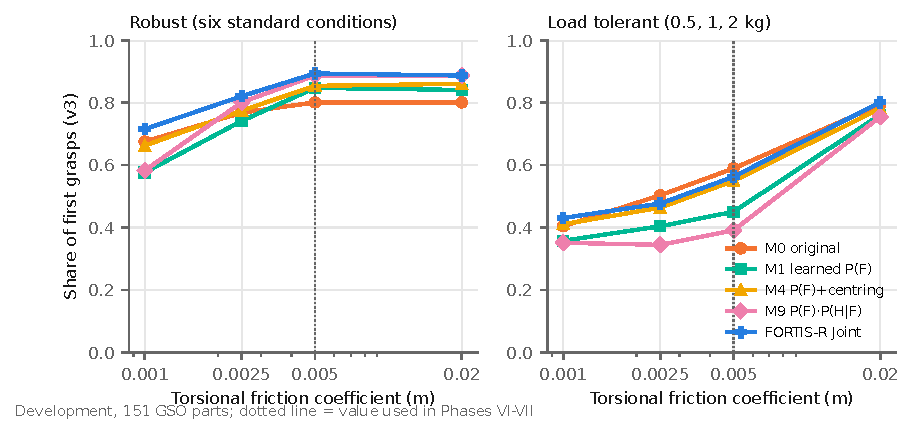
\includegraphics[width=\textwidth]{figures/fig_dev_torsion.pdf}
\caption{Development: robustness and load tolerance of each method's first viable grasp across the torsional-friction grid (v3 criterion, \devParts{} GSO parts). Rankings in robustness are stable above 0.0025~m; load tolerance depends strongly on the uncalibrated parameter.}\label{fig:torsion}
\end{figure}

\section{Methods}\label{sec:methods}

Let $P(F\mid g)$ be a classifier of feasibility for candidate $g$ and $\tilde p = P(F\mid g)/\max_{g'} P(F\mid g')$ its per-object normalisation. Let $P(H\mid F, g)$ be the probability that a feasible candidate is dynamically robust, and $Q_{cen}\in[0,1]$ the planner's centring term (one minus the lever arm between the closing line and the centre of mass, relative to the finger depth). All orders keep the stroke gate.
\begin{itemize}
\item \textbf{M0} (original planner): no prior.
\item \textbf{M1} (learned feasibility): prior $\tilde p$ with $w=2$.
\item \textbf{M4}: order by $\tilde p^{0.8}\,Q_{cen}^{0.2}$.
\item \textbf{M9}: order by $\tilde p\cdot P(H\mid F)$.
\item \textbf{FORTIS-R Joint} (final method): order by $\tilde p\cdot P(H\mid F)\cdot \max(Q_{cen},10^{-3})^{\beta}$ with $\beta=0.3$.
\end{itemize}
Fusion orders are passed to the native planner as encoded priors. $P(F)$ is gradient boosting \cite{pedregosa2011sklearn} on 19 candidate features (approach and closing directions, width, relative position, height, log extents, antipodality, centre offset, preliminary score, makeability); $P(H\mid F)$ is gradient boosting on the same features with the robust label. $\beta$ was chosen among $\{0.1,0.2,0.3,0.5\}$ by a criterion fixed in advance (standardised mean log $N_{FR}$ plus the share of first grasps that are not load tolerant), in nested cross-validation and on all development parts (0.3 in both).

\paragraph{Fallback with a guarantee.} A learned order can be worse than the original on some objects (negative transfer). Interleaving the learned order $L$ and the original order $D$ ($L_1, D_1, L_2, D_2,\dots$, skipping candidates already examined) bounds the cost: after $2m$ steps the first $m$ candidates of both orders have been examined, so
\begin{equation}
N_{\text{hybrid}} \le 2\min(N_L, N_D),
\end{equation}
and with $k$ orders in round robin $N\le k\min_i N_i$. The bound needs no assumption about the prior.

\section{Development study}\label{sec:dev}

\paragraph{Data and splits.} Development used \devAllParts{} parts: 116 library parts (16 YCB, 100 GSO \cite{downs2022gso}) and 200 GSO test parts from earlier phases, of which \devParts{} have a viable grasp and dynamic labels. Representation models used 5-fold cross-validation grouped by product name; robustness models used the earlier phase's 5 outer folds. All development results are out of fold and are \emph{not} confirmatory.

\paragraph{Order and robustness.} Table~\ref{tab:dev} shows the trade-off. The learned order reduces $N_F$ from \devNFMzero{} to \devNFMone, but its first grasps are less load tolerant than the original planner's (\devLoadMone\% vs \devLoadMzero\%). FORTIS-R Joint keeps the learned efficiency ($N_F$ \devNFJoint) and is more robust than the original planner (\devJointMzeroRobust{} percentage points, 95\% CI \devJointMzeroRobustCI), with load tolerance close to it (\devJointMzeroLoad, \devJointMzeroLoadCI). With the articulated arm, the robustness gain is preserved (\artJointMzeroRobust, \artJointMzeroRobustCI) but the load contrasts reverse: Joint$-$M1 load tolerance is \devJointMoneLoad{} percentage points with the floating palm and \artJointMoneLoad{} \artJointMoneLoadCI{} with the arm (Fig.~\ref{fig:articulated}). For this reason load tolerance was excluded from the primary confirmatory family.

\begin{table}[t]
\caption{Development (\devParts{} GSO parts, out of fold): geometric-mean $N_F$ and the share of first viable grasps that are robust or load tolerant under the corrected (v3) and the previous (v2) criteria; torsion 0.005~m.}\label{tab:dev}
\centering\small
% Generated by make_tables.py
\begin{tabular}{lrrrrr}
\toprule
Method & $N_F$ & Robust v3 (\%) & Load v3 (\%) & Robust v2 (\%) & Load v2 (\%) \\
\midrule
M0 original planner & 6.07 & 80.1 & 58.9 & 84.1 & 64.9 \\
M1 learned $P(F)$ & 1.25 & 84.8 & 45.0 & 90.7 & 48.3 \\
M4 $\tilde p^{0.8} Q_{cen}^{0.2}$ & 1.23 & 85.4 & 55.0 & 92.7 & 60.3 \\
M9 $\tilde p\,P(H|F)$ & 1.29 & 88.7 & 39.1 & 96.0 & 46.4 \\
FORTIS-R Joint & 1.29 & 89.4 & 56.3 & 96.7 & 62.3 \\
\bottomrule
\end{tabular}

\end{table}

\begin{figure}[t]
\centering
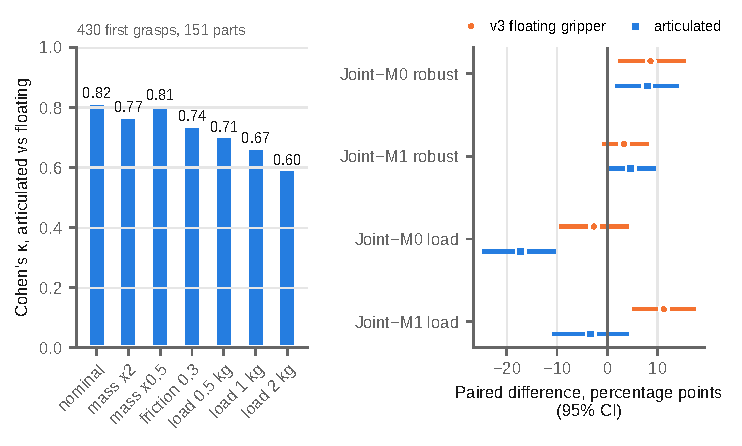
\includegraphics[width=\textwidth]{figures/fig_dev_articulated.pdf}
\caption{Development: agreement between the floating-gripper test and the articulated-arm replication by condition (left), and the main contrasts at both levels (right, paired differences with 95\% bootstrap CIs). The levels agree in standard conditions and disagree under heavy loads.}\label{fig:articulated}
\end{figure}

\paragraph{Negative transfer.} The learned orders are worse than the original on few objects but sometimes by a lot: M1 on \devNegMone{} parts (worst ratio \devWorstMone), FORTIS-R Joint on \devNegJoint{} (worst \devWorstJoint). Interleaving Joint with M0 caps the worst ratio at \devHybridWorst{} with a geometric-mean $N_F$ of \devHybridNF.

\paragraph{Representations.} We compared gradient boosting (L0), logistic regression and a three-branch MLP (candidate, geometry---log extents and the D2 shape distribution \cite{osada2002shape}---and vision) with frozen DINOv2, DINOv3 and OpenCLIP descriptors (unit mean of 16 grey renders), an untrained ViT, permuted embeddings and linear visual branches (Table~\ref{tab:rep}, Fig.~\ref{fig:rep}). Gradient boosting was the best ($N_F$ \repNFLzero, AUC \repAUCLzero); the geometry MLP needed \repLtwoLzero{} times as many candidates \repLtwoLzeroCI. Adding DINOv3 through a nonlinear branch did not help (\repLeightLtwo{} \repLeightLtwoCI) and did not differ from its permuted control (\repLeightPerm{} \repLeightPermCI). A linear DINOv3 branch (L10) was the best visual variant (\repLtenLtwo{} \repLtenLtwoCI{} vs the geometry MLP; \repLtenPerm{} \repLtenPermCI{} vs its permuted control, a control added after L10's result was seen); neither interval survives Holm correction, so no visual representation met the pre-declared development rule. DINOv3 patch tokens sampled at the contacts (\repVisibleShare\% of contacts visible after snapping to the render surface) and classical local geometry behaved alike (\repLDLtwo{} and \repLGLtwo). A listwise ranking loss \cite{cao2007listnet} did not help (\repRankLtwo{} \repRankLtwoCI).

\begin{figure}[t]
\centering
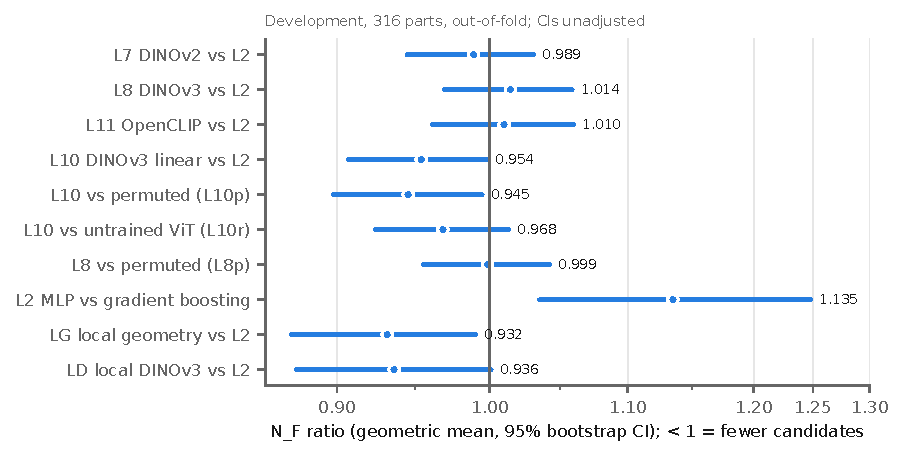
\includegraphics[width=0.85\textwidth]{figures/fig_dev_representation.pdf}
\caption{Development: $N_F$ ratios between representation variants (geometric mean over \devAllParts{} parts, out of fold, 95\% bootstrap CIs, unadjusted). Values below 1 mean fewer examined candidates.}\label{fig:rep}
\end{figure}

\begin{table}[t]
\caption{Development representation benchmark (\devAllParts{} parts, out of fold, MLPs averaged over three seeds). S@1: share of all parts whose first examined candidate is viable; Robust: share of robust first grasps (v2 labels) on the \devParts{} dynamic parts. $^\dagger$Added after L10's result was seen.}\label{tab:rep}
\centering\scriptsize
% Generated by make_tables.py
\begin{tabular}{llrrrrr}
\toprule
Id & Model & AUC & ECE & $N_F$ & S@1 & Robust \\
\midrule
L0 & Gradient boosting, 19 features & 0.9958 & 0.0030 & 1.316 & 0.642 & 0.927 \\
L1 & Logistic regression & 0.9846 & 0.0046 & 1.890 & 0.525 & 0.947 \\
L2v & MLP, candidate only & 0.9944 & 0.0022 & 1.491 & 0.606 & 0.903 \\
L2 & MLP, + geometry $u$ & 0.9755 & 0.0194 & 1.494 & 0.599 & 0.903 \\
L3 & MLP, + DINOv2 (linear) & 0.9945 & 0.0039 & 1.422 & 0.612 & 0.879 \\
L4 & MLP, + DINOv3 (linear) & 0.9939 & 0.0043 & 1.422 & 0.611 & 0.890 \\
L5 & MLP, + DINOv2 & 0.9945 & 0.0033 & 1.417 & 0.614 & 0.912 \\
L6 & MLP, + DINOv3 & 0.9941 & 0.0035 & 1.465 & 0.599 & 0.901 \\
L7 & MLP, $u$ + DINOv2 & 0.9664 & 0.0287 & 1.478 & 0.595 & 0.901 \\
L8 & MLP, $u$ + DINOv3 & 0.9661 & 0.0291 & 1.516 & 0.580 & 0.894 \\
L9 & MLP, $u$ + untrained ViT & 0.9933 & 0.0038 & 1.472 & 0.606 & 0.883 \\
L10 & MLP, $u$ + DINOv3 (linear) & 0.9752 & 0.0205 & 1.425 & 0.611 & 0.901 \\
L10p & L10 with permuted DINOv3$^\dagger$ & 0.9919 & 0.0058 & 1.508 & 0.593 & 0.907 \\
L10r & L10 with untrained ViT$^\dagger$ & 0.9852 & 0.0120 & 1.472 & 0.602 & 0.890 \\
L8p & L8 with permuted DINOv3 & 0.9922 & 0.0048 & 1.518 & 0.595 & 0.914 \\
L11 & MLP, $u$ + OpenCLIP & 0.9657 & 0.0298 & 1.509 & 0.595 & 0.892 \\
LG & MLP, $u$ + local geometry & 0.9837 & 0.0136 & 1.392 & 0.611 & 0.846 \\
LD & MLP, $u$ + local DINOv3 & 0.9741 & 0.0228 & 1.399 & 0.612 & 0.868 \\
LGD & MLP, $u$ + both local & 0.9633 & 0.0315 & 1.441 & 0.594 & 0.896 \\
L2-rank & L2, listwise loss & 0.9887 & 0.0110 & 1.505 & 0.587 & 0.854 \\
L8-rank & L8, listwise loss & 0.9882 & 0.0099 & 1.540 & 0.577 & 0.879 \\
\bottomrule
\end{tabular}

\end{table}

\paragraph{Room for adaptation.} With the learned order, the first examined candidate is viable for \fewFirstShare\% of development parts. A perfect adaptive model could therefore save on average \fewCeiling{} candidates per part (about \fewCeilingMs~ms of planner time) against a fixed cost of \fewFixedS~s per call, before paying for its own support evaluations. Few-shot adaptation, deep kernel learning and ADKF-IFT \cite{wilson2016dkl,chen2023adkfift} were therefore not run.

\paragraph{Other grippers.} A feasibility model trained at 80~mm and applied zero-shot to 40~mm and 120~mm catalogues of the same parts needed \crossForty{} \crossFortyCI{} and \crossHundredtwenty{} \crossHundredtwentyCI{} times as many candidates as models trained for those grippers (\crossFortyViable{} and \crossHundredtwentyViable{} viable parts). These are separate configurations of one cell, not different robots.

%% Confirmatory study. Numbers: tables/numbers.tex (generated from research/phase7/results/confirmation_results.json).
\section{Confirmatory study on EGAD}\label{sec:conf}

\paragraph{Design, frozen before opening.} The confirmatory set was drawn from the EGAD training set \cite{morrison2020egad}: one mesh per grid cell (difficulty $\times$ complexity), in a seeded order fixed by metadata and watertightness checks alone; the first \confObjects{} positions form the primary set and the 45 accepted evaluation-set objects a secondary set. Meshes were scaled with the dataset authors' rule for an 80~mm gripper, placed on their most probable stable face and decomposed for collision with CoACD \cite{wei2022coacd}; the decomposition settings were chosen on three objects outside the confirmatory positions. Before any confirmatory object was planned, the protocol, the frozen models ($P(F)$ refitted on all \devAllParts{} development parts, $P(H\mid F)$ on the \devParts{} dynamic ones, $\beta=0.3$), the hypotheses, the sample size (from paired power simulations on development data) and the analysis code were committed and signed by SHA-256 hashes. Two disclosed deviations: the cells of two primary objects were built (geometry only) while the pipeline was written, and the choice of the H5 representation and the move of load tolerance to the secondary family were made after development results (Sect.~\ref{sec:dev}).

\paragraph{Hypotheses and statistics.} The primary family (Holm, one-sided familywise $\alpha=0.025$, paired by object) was: P1, Joint examines fewer candidates than the original planner ($N_F$ ratio $<1$, Wilcoxon signed-rank \cite{wilcoxon1945}); P2, Joint's v3 robustness is non-inferior to the original planner's with a 5-percentage-point margin, followed---only if P2 holds---by a superiority test at $0.025/3$ (exact McNemar \cite{mcnemar1947}); P3, Joint's $N_F$ is non-inferior to the best learned baseline M1 with a ratio margin of 1.25. Seven secondary hypotheses (Holm \cite{holm1979}) covered the historical H1 and H2, load tolerance, the full online cost (H4) and the representation question (H5). Effect sizes are reported with paired bootstrap 95\% CIs \cite{efron1979bootstrap}.

\paragraph{Objects.} Of the \confObjects{} primary objects, \confViable{} (\confViableShare\%) had at least one viable candidate and \confNonViable{} had none; all \confViable{} viable objects have dynamics. Over all \confObjects{} objects, the share with a grasp at the first examined candidate was \confSoneMzero\% for the original planner and \confSoneJoint\% for FORTIS-R Joint, and within 50 candidates \confSfiftyMzero\% and \confSfiftyJoint\% (Fig.~\ref{fig:success}).

\paragraph{Primary results.} Table~\ref{tab:conf} and Fig.~\ref{fig:conf} give the outcomes. \textbf{P1} was \confPoneVerdict: Joint examined \confPoneRatio{} times as many candidates as the original planner \confPoneCI, a smaller gain than in development because the original planner is far more efficient on EGAD ($N_F$ \confNFMzero{} vs \devNFMzero). \textbf{P2} was \confPtwoVerdict, narrowly: the robustness difference was \confPtwoDiff{} percentage points \confPtwoCI, with the one-sided 97.5\% lower limit at \confPtwoLower{} against the $-5$ margin. Superiority was \confPtwoSupVerdict{} (discordant objects \confPtwoSupFav{} in favour, \confPtwoSupUnfav{} against): the development robustness gain did not replicate. \textbf{P3} was \confPthreeVerdict: Joint and M1 examined the same number of candidates (ratio \confPthreeRatio{} \confPthreeCI).

\begin{table}[t]
\caption{Primary confirmatory family on the EGAD primary set (\confViable{} viable objects). Effects: $N_F$ ratios or paired differences in percentage points, with 95\% bootstrap CIs; Holm-adjusted one-sided $p$; ``supported'' also requires the CI or bound criterion of the protocol.}\label{tab:conf}
\centering\scriptsize
% Generated by make_tables.py
\begin{tabular}{p{0.08\textwidth}p{0.42\textwidth}lrr}
\toprule
Id & Hypothesis & Effect (95\% CI) & Holm $p$ & Supported \\
\midrule
P1 & FORTIS-R Joint examines fewer candidates than the original planner ($N_F$ ratio $<$ 1) & 0.609 [0.516, 0.711] & $<10^{-4}$ & yes \\
P2 & Joint robustness (v3) non-inferior to the original planner, margin 5 pp & $-$1.8 [$-$5.0, 1.4] & 0.022 & yes \\
P3 (H3) & Joint $N_F$ non-inferior to the best learned baseline M1, ratio margin 1.25 & 0.993 [0.953, 1.037] & $<10^{-4}$ & yes \\
P2-sup & Joint more robust than M0 (only if P2) & $-$1.8 [$-$5.0, 1.4] & 0.93 & no \\
\bottomrule
\end{tabular}

\end{table}

\begin{figure}[t]
\centering
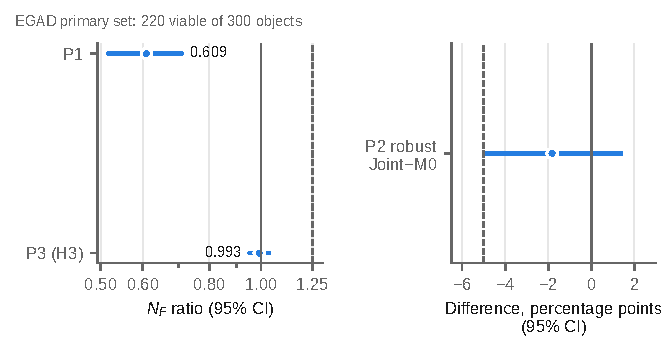
\includegraphics[width=\textwidth]{figures/fig_conf_primary.pdf}
\caption{Primary confirmatory contrasts on EGAD. Left: $N_F$ ratios (P1: Joint vs original planner; P3: Joint vs M1, dashed line = non-inferiority margin 1.25). Right: robustness difference Joint$-$M0 (dashed line = margin $-5$ percentage points).}\label{fig:conf}
\end{figure}

\paragraph{Secondary results.} None of the seven secondary hypotheses was supported (Supplementary Table~S2). The historical hypotheses did not replicate: M4 and M1 had the same load tolerance (\confSSoneEff), and M9 was not more robust than M1 (\confSStwoEff). Joint and M1 had the same load tolerance and robustness (\confSSthreeEff{} and \confSSfourEff). Joint was \emph{less} load tolerant than the original planner (\confSSfiveEff, failing the 10-point non-inferiority margin), the direction the articulated development pilot had suggested. The full online cost of Joint was \confSSsixEff{} times the original planner's (H4, Sect.~\ref{sec:cost}). The DINOv3 linear-branch MLP did not examine fewer candidates than the geometry MLP (\confSSsevenEff) nor than its permuted control (\confHfivePerm{} \confHfivePermCI); H5 was \confHfiveSupported.

\paragraph{Sensitivity.} The robustness non-inferiority holds only at the pre-registered torsional friction: the Joint$-$M0 robustness difference was \confTorLowPtwo{} \confTorLowPtwoCI{} at 0.001~m and \confTorHighPtwo{} \confTorHighPtwoCI{} at 0.02~m, both below zero. Across rotation thresholds it was \confRotFivePtwo{} (5$^\circ$), \confRotTenPtwo{} (10$^\circ$) and \confRotTwentyPtwo{} (20$^\circ$). With the articulated arm (\confArtObjects{} objects), Joint$-$M0 was \confArtJointMzeroRobust{} \confArtJointMzeroRobustCI{} in robustness (four standard conditions) and \confArtJointMzeroLoad{} \confArtJointMzeroLoadCI{} in load tolerance.

\paragraph{Fallback and negative transfer.} Joint examined more candidates than the original planner on \confNegJoint{} viable objects; the round-robin hybrid never exceeded twice the original planner's cost (\confHybridViol{} violations of the bound) and had geometric-mean $N_F$ \confHybridNF.

\paragraph{Evaluation set.} On the \evalViable{} viable of the \evalObjects{} EGAD evaluation-set objects (reported separately, not part of either family), Joint needed \evalNFJoint{} candidates against \evalNFMzero{} for the original planner, with equal robustness (\evalRobustJoint\% and \evalRobustMzero\%).

\begin{figure}[t]
\centering
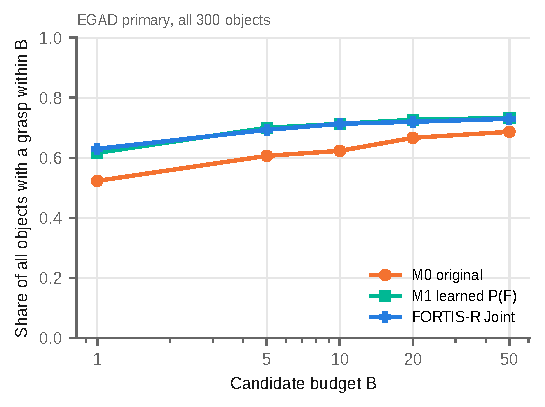
\includegraphics[width=0.55\textwidth]{figures/fig_conf_success_at_budget.pdf}
\caption{EGAD primary set, all \confObjects{} objects: share of objects for which a viable grasp is found within a budget of $B$ examined candidates. Objects without any viable candidate count as failures for every method.}\label{fig:success}
\end{figure}

\begin{table}[t]
\caption{EGAD primary set: all methods. $N_F$ on viable objects; S@1 and S@10 over all objects; v3 rates on viable objects with dynamics.}\label{tab:confmethods}
\centering\small
% Generated by make_tables.py
\begin{tabular}{lrrrrr}
\toprule
Method & $N_F$ & S@1 (\%) & S@10 (\%) & Robust v3 (\%) & Load v3 (\%) \\
\midrule
M0 & 2.09 & 52.3 & 62.3 & 92.7 & 85.0 \\
M1 & 1.28 & 61.7 & 71.3 & 91.8 & 77.7 \\
M4 & 1.29 & 62.7 & 71.0 & 90.0 & 77.7 \\
M9 & 1.26 & 62.3 & 72.0 & 90.9 & 75.4 \\
Joint & 1.27 & 63.0 & 71.3 & 90.9 & 78.6 \\
\bottomrule
\end{tabular}

\end{table}

\section{Online cost}\label{sec:cost}

The planner reports its own stage timings, and the full pipeline was timed from receiving an object to the planner's answer, with one thread and nothing else running. In the current implementation the learned orders need the candidates before planning, so candidate generation runs twice: once in a separate export process and once inside the planner. On \timeObjects{} confirmatory objects the median full cost was \timeMzero~s for the original planner and \timeJoint~s for Joint. Generation alone took \timeGen~s, whereas the search stage that the order accelerates took \timeSearchMzero~ms (original) and \timeSearchJoint~ms (Joint); every first grasp of the timed runs matched the order replay (\timeMismatch{} mismatches). On \costParts{} development parts the full-cost ratio was \costJointTotal{} \costJointTotalCI; subtracting the duplicated generation---an engineering estimate of a single-process implementation, not a measurement---gives \costJointIntegrated{} \costJointIntegratedCI. A visual prior would add rendering (\costDinoRender~s median for 16 views on CPU) and encoding (\costDinoEncode~s). The classical analytic order (force closure, then wrench-space quality \cite{ferrari1992planning}), evaluated on \epsParts{} development parts, needed \epsNF{} candidates against \epsNFMzero{} for the original planner and \epsNFJoint{} for Joint, and its quality export took \epsSeconds~s per part.


\section{Discussion}\label{sec:discussion}

%% Discussion. Numbers: tables/numbers.tex.
\paragraph{What the independent test confirmed.} A feasibility classifier trained on household scans transferred to evolved shapes it had never seen: the learned order examined fewer candidates than the original planner (P1), and adding the robustness and centring terms cost nothing in efficiency relative to the plain learned order (P3). The gain was smaller than in development (\confPoneRatio{} vs \devPoneRatio), because the original planner's heuristic order is already good on gripper-scaled EGAD shapes. The population-level view matters here: \confNonViable{} of \confObjects{} objects had no viable candidate at all, and no ordering can change that.

\paragraph{What it did not confirm.} The robustness advantage that motivated FORTIS-R Joint in development (\devJointMzeroRobust{} points) did not replicate; on EGAD Joint was non-inferior to the original planner only at the pre-registered friction value, narrowly, and fell below it at the other torsional-friction values. Load tolerance was lower than the original planner's. The historical claims that a centring term improves load tolerance (H1) and that a learned robustness model improves robustness (H2) also failed to replicate. Two explanations are consistent with the data, and the study cannot separate them: the robustness model was trained on development labels from a different population (household scans, the previous rise-and-slip criterion), and the original planner's grasps are already highly robust on EGAD (\confRobustMzero\%), leaving little room. Either way, a robustness term learned on one object population should not be assumed to help on another.

\paragraph{Physics modelling decides load-tolerance conclusions.} Two choices that are rarely reported changed conclusions: the torsional friction coefficient (between \devFlipHigh\% and \devFlipLow\% of verdicts changed over the tested range) and whether the gripper floats or hangs from an articulated arm (load contrasts reversed between the two in development). Moving load tolerance out of the primary family before the test was justified by these development results; the confirmation then agreed with the articulated direction. Claims about load tolerance from a single floating-gripper simulation should be treated with caution.

\paragraph{Efficiency in candidates is not efficiency in seconds.} For this planner, generating the catalogue costs several times more than searching it, and the learned order only shortens the search. With the present two-process implementation the learned orders were roughly twice as slow end to end (H4 failed). Integrating the prior into the planner removes the duplicated generation; our estimate of that implementation is close to parity with the original planner, not faster. The number of examined candidates remains the right measure when candidate evaluation is expensive (e.g. with full motion planning or physics in the loop), but the claim of a wall-clock saving does not hold here.

\paragraph{Foundation-model features.} Frozen DINOv2, DINOv3 and OpenCLIP global descriptors, DINOv3 patch tokens at the contacts, and a listwise ranking loss did not improve on a gradient-boosting model over 19 hand-designed candidate features, in development or confirmation, once permuted and untrained controls were considered. With the learned order the first examined candidate is already viable for most objects, so there is little left for richer object descriptors---or for few-shot adaptation---to gain. This is a bounded negative result: it concerns frozen descriptors of grey renders for ordering a planner's candidates, not visual grasp learning in general.

\paragraph{Practical guidance.} For a complete sampling-based planner: (i) learn the examination order from exhaustively labelled catalogues and evaluate it with an exact replay of the planner; (ii) run it in round robin with the original order to bound the worst case at twice the original cost; (iii) validate dynamic claims across friction and simulator-fidelity variations and on an independent population before relying on a learned robustness term; (iv) measure end-to-end time, not only examined candidates.

\paragraph{Limitations.} Everything is simulated, with assumed masses, uniform density and uncalibrated friction; no real robot was used. One cell and one 80~mm gripper were confirmed; the 40 and 120~mm results are development-only stroke variants. EGAD shapes are gripper-scaled evolved objects, not household items, and their collision geometry is a convex decomposition. The articulated model uses the cell's link inertias and an ideal computed-torque controller without arm collisions. No learned external grasp detector was reproduced (GPD would need a C++ adapter; Contact-GraspNet a GPU; Dex-Net a legacy software stack); the only external comparison is a reimplemented analytic criterion. Two secondary hypotheses (H2 in particular) were underpowered, and non-significant results there are not evidence of equivalence.


\section{Conclusion}\label{sec:conclusion}

%% Conclusion. Numbers: tables/numbers.tex.
We measured, under a pre-registered and hash-signed protocol, what a learned examination order does to a complete parallel-jaw grasp planner. On an independent set of \confObjects{} EGAD objects, FORTIS-R Joint examined \confPoneRatio{} times as many candidates as the original planner and as few as the plain learned order, with a round-robin fallback that never exceeded twice the original cost. Its robustness was only narrowly non-inferior to the original planner and depended on uncalibrated friction; the robustness and load-tolerance gains seen in development did not replicate, and the end-to-end cost of the current implementation was higher than the original planner's. Frozen vision foundation-model features added nothing measurable. The defensible message is a cautious one: learned ordering reliably saves planner evaluations across object populations, but robustness benefits learned on one population, and conclusions drawn from a single simulator configuration, need independent confirmation---which, here, they did not receive. Real-robot experiments, calibrated contact parameters and an integrated implementation are the necessary next steps.


\backmatter

\bmhead{Supplementary information} The supplementary material (supplementary.tex) contains the full development tables, the protocol, the frozen hypotheses and the secondary analyses.

\bmhead{Acknowledgements} [To be completed by the author.]

\section*{Declarations}

\begin{itemize}
\item \textbf{Funding} [To be completed by the author. No funding is recorded in the repository.]
\item \textbf{Competing interests} [To be completed by the author.]
\item \textbf{Ethics approval and consent to participate} Not applicable: no human or animal participants.
\item \textbf{Consent for publication} Not applicable.
\item \textbf{Data availability} See data\_availability.md. EGAD (BSD-3) and Google Scanned Objects (CC BY 4.0) are public; derived catalogues, results and protocols are in the project repository.
\item \textbf{Materials availability} Not applicable.
\item \textbf{Code availability} See code\_availability.md.
\item \textbf{Author contribution} E.P.G. conceived the study and is responsible for the work. Use of AI tools is described in ai\_usage\_disclosure.md.
\item \textbf{Use of generative AI} Claude Code (Anthropic) and ChatGPT (OpenAI) were used as described in the AI-usage disclosure; they are not authors.
\end{itemize}

\bibliography{references}

\end{document}
